\PassOptionsToPackage{unicode=true}{hyperref} % options for packages loaded elsewhere
\PassOptionsToPackage{hyphens}{url}
\PassOptionsToPackage{dvipsnames,svgnames*,x11names*}{xcolor}
%
\documentclass[10pt,dvipsnames]{scrartcl}
\usepackage{lmodern}
\usepackage{amssymb,amsmath}
\usepackage{ifxetex,ifluatex}
\usepackage{fixltx2e} % provides \textsubscript
\ifnum 0\ifxetex 1\fi\ifluatex 1\fi=0 % if pdftex
  \usepackage[T1]{fontenc}
  \usepackage[utf8]{inputenc}
  \usepackage{textcomp} % provides euro and other symbols
\else % if luatex or xelatex
  \usepackage{unicode-math}
  \defaultfontfeatures{Ligatures=TeX,Scale=MatchLowercase}
\fi
% use upquote if available, for straight quotes in verbatim environments
\IfFileExists{upquote.sty}{\usepackage{upquote}}{}
% use microtype if available
\IfFileExists{microtype.sty}{%
\usepackage[]{microtype}
\UseMicrotypeSet[protrusion]{basicmath} % disable protrusion for tt fonts
}{}
\IfFileExists{parskip.sty}{%
\usepackage{parskip}
}{% else
\setlength{\parindent}{0pt}
\setlength{\parskip}{6pt plus 2pt minus 1pt}
}
\usepackage{xcolor}
\usepackage{hyperref}
\hypersetup{
            pdftitle={Burdens of Proof - Sample Chapter},
            pdfauthor={Marcello Di Bello and Rafal Urbaniak},
            colorlinks=true,
            linkcolor=Maroon,
            filecolor=Maroon,
            citecolor=Blue,
            urlcolor=blue,
            breaklinks=true}
\urlstyle{same}  % don't use monospace font for urls
\usepackage{graphicx,grffile}
\makeatletter
\def\maxwidth{\ifdim\Gin@nat@width>\linewidth\linewidth\else\Gin@nat@width\fi}
\def\maxheight{\ifdim\Gin@nat@height>\textheight\textheight\else\Gin@nat@height\fi}
\makeatother
% Scale images if necessary, so that they will not overflow the page
% margins by default, and it is still possible to overwrite the defaults
% using explicit options in \includegraphics[width, height, ...]{}
\setkeys{Gin}{width=\maxwidth,height=\maxheight,keepaspectratio}
\setlength{\emergencystretch}{3em}  % prevent overfull lines
\providecommand{\tightlist}{%
  \setlength{\itemsep}{0pt}\setlength{\parskip}{0pt}}
\setcounter{secnumdepth}{5}
% Redefines (sub)paragraphs to behave more like sections
\ifx\paragraph\undefined\else
\let\oldparagraph\paragraph
\renewcommand{\paragraph}[1]{\oldparagraph{#1}\mbox{}}
\fi
\ifx\subparagraph\undefined\else
\let\oldsubparagraph\subparagraph
\renewcommand{\subparagraph}[1]{\oldsubparagraph{#1}\mbox{}}
\fi

% set default figure placement to htbp
\makeatletter
\def\fps@figure{htbp}
\makeatother

%\documentclass{article}

% %packages
 \usepackage{booktabs}


\usepackage{graphicx}
\usepackage{longtable}
\usepackage{ragged2e}
\usepackage{etex}
%\usepackage{yfonts}
\usepackage{marvosym}
\usepackage[notextcomp]{kpfonts}
\usepackage{nicefrac}
\newcommand*{\QED}{\hfill \footnotesize {\sc Q.e.d.}}

\usepackage[textsize=footnotesize]{todonotes}
%\linespread{1.5}


\setlength{\parindent}{10pt}
\setlength{\parskip}{1pt}


%language
\usepackage{times}
\usepackage{t1enc}
%\usepackage[utf8x]{inputenc}
%\usepackage[polish]{babel}
%\usepackage{polski}




%AMS
\usepackage{amsfonts}
\usepackage{amssymb}
\usepackage{amsthm}
\usepackage{amsmath}

\usepackage{geometry}
 \geometry{a4paper,left=35mm,top=20mm,}

%abbreviations
\newcommand{\ra}{\rangle}
\newcommand{\la}{\langle}
\newcommand{\n}{\neg}
\newcommand{\et}{\wedge}
\newcommand{\jt}{\rightarrow}
\newcommand{\ko}[1]{\forall  #1\,}
\newcommand{\ro}{\leftrightarrow}
\newcommand{\exi}[1]{\exists\, {_{#1}}}
\newcommand{\pr}{\mathsf{P}}
\newcommand{\odds}{\mathsf{Odds}}
\newcommand{\ind}{\mathsf{Ind}}
\newcommand{\nf}[2]{\nicefrac{#1\,}{#2}}
\newcommand{\R}[1]{\texttt{#1}}

\newtheorem{q}{\color{blue}Question}
\newtheorem{lemma}{Lemma}
\newtheorem{theorem}{Theorem}




\newtheorem*{reply*}{Reply}
\usepackage{enumitem}
\newcommand{\question}[1]{\begin{enumerate}[resume,leftmargin=0cm,labelsep=0cm,align=left]
\item #1
\end{enumerate}}

\usepackage{float}

% \setbeamertemplate{blocks}[rounded][shadow=true]
% \setbeamertemplate{itemize items}[ball]
% \AtBeginPart{}
% \AtBeginSection{}
% \AtBeginSubsection{}
% \AtBeginSubsubsection{}
% \setlength{\emergencystretch}{0em}
% \setlength{\parskip}{0pt}






\usepackage[authoryear]{natbib}

%\bibliographystyle{apalike}

\title{Burdens of Proof - Sample Chapter}
\author{Marcello Di Bello and Rafal Urbaniak}
\date{}

\begin{document}
\maketitle

\tableofcontents

\hypertarget{sample-chapter---introduction}{%
\section{SAMPLE CHAPTER -
Introduction}\label{sample-chapter---introduction}}

After the evidence has been presented, examined and cross-examined at
trial, trained judges or lay jurors must reach a decision. The decision
criterion is defined by law and consists of a standard of proof, also
called the burden of persuasion. So long as the evidence against the
defendant is sufficiently strong to meet the requisite proof standard,
the defendant should be found liable. This chapter begins with a
description of standards of proof in the law, then outlines different
probabilistic approaches, discusses challanges to these approaches,
compares them with competing accounts in the literature.

\hypertarget{legal-background}{%
\section{Legal Background}\label{legal-background}}

\label{subsec:legal-background}

\hypertarget{burden-of-pleading-production-and-persuasion}{%
\subsection{Burden of pleading, production and
persuasion}\label{burden-of-pleading-production-and-persuasion}}

\hypertarget{proof-standards-in-the-law}{%
\subsection{Proof standards in the
law}\label{proof-standards-in-the-law}}

In criminal proceedings, the governing standard is `proof beyond a
reasonable doubt.' If the decision makers are persuaded beyond a
reasonable doubt that the defendant is guilty, they should convict, or
else they should acquit. In civil cases, the standard is typically
`preponderance of the evidence'. The latter is less demanding than the
former, so the same body of evidence may be enough to meet the
preponderance standard, but not enough to meet the beyond a reasonable
doubt standard. A vivid example of this difference is the 1995 trial of
O.J. Simpson who was charged with murdering his wife. He was acquitted
of the criminal charges, but when the family of the victim brought a
lawsuit against him, they prevailed. O.J.~Simpson did not kill his wife
according to the beyond a reasonable doubt standard, but he did
according to the preponderance standard. An intermediate standard,
called `clear and convincing evidence', is sometimes used for civil
proceedings in which the decision is particularly weighty, for example,
a decision whether someone should be committed to a hospital facility.

This tripartite distinction of proof standards---beyond a reasonable
doubt; preponderance; clear and convincing evidence---is common in
Anglo-american jurisprudence. It is not universal, however. Different
countries may use different standards. France, for example, uses the
standard of `intimate conviction' for both civil and criminal
proceedings. Judges deciding cases `must search their conscience in good
faith and silently and thoughtfully ask themselves what impression the
evidence given against the accused and the defence's arguments have made
upon them' (French Code of Criminal Procedure, art.~353). German law is
similar. Germany's Code of Civil Procedure, Sec.~286, states that `it is
for the court to decide, based on its personal conviction, whether a
factual claim is indeed true or not.'

How to define standards of proof, or whether they should be even defined
in the first place, remains contentious (Diamond, 1990; Horowitz \&
Kirkpatrick, 1996; Laudan, 2006; Newman, 1993; Walen, 2015). Judicial
opinions offer different paraphrases, sometimes conflicting, of what
these standards mean. The meaning of `proof beyond a reasonable doubt'
is the most controversial. It has been equated to `moral certainty' or
`abiding conviction' (Commonwealth v. Webster, 59 Mass. 295, 320, 1850)
or to `proof of such a convincing character that a reasonable person
would not hesitate to rely and act upon it in the most important of his
own affairs' (US Federal Jury Practice and Instructions, 12.10, at 354,
4th ed.~1987). But courts have also cautioned that there is no need to
define the term because `jurors know what is reasonable and are quite
familiar with the meaning of doubt' and attempts to define it only
`muddy the water' (U.S. v. Glass, 846 F.2d 386, 1988).

Probability theory can bring conceptual clarity to an otherwise
heterogeneous legal doctrine, or at least this is the position of legal
probabilists.

\hypertarget{probabilistic-thresholds}{%
\section{Probabilistic Thresholds}\label{probabilistic-thresholds}}

\hypertarget{posterior-probability-kaplan-kaye-etc.}{%
\subsection{Posterior probability (Kaplan, Kaye,
etc.)}\label{posterior-probability-kaplan-kaye-etc.}}

Legal probabilists have proposed to interpret proof beyond a reasonable
doubt as the requirement that the defendant's probability of guilt,
given the evidence presented at trial, meet a threshold, say,
\textgreater{}95\%. Variations of this view are common (see Bernoulli,
1713; Dekay, 1996; Kaye, 1979a; Laplace, 1814, @Kaplan1968decision;
Laudan, 2006). This interpretation is, in some respects, plausible. From
a legal standpoint, the requirement that guilt be established with high
probability, still short of 100\%, accords with the principle that proof
beyond a reasonable doubt is the most stringent standard of all but at
the same time `does not involve proof to an absolute certainty' and thus
`it is not proof beyond any doubt' (R v Lifchus, 1997, 3 SCR 320, 335).
That this intepretation is quite natural is further attested by the fact
that the probabilistic interpretation is taken for granted in
psychological studies about people's understanding of proof beyond a
reasonable doubt (Dhami, Lundrigan, \& Mueller-Johnson, 2015). This
research examines whether people use a 75\% or 95\% threshold, and does
not question whether the standard functions as a probabilistic
threshold.

Reliance on probabilistic ideas is even more explicit in the standard
`preponderance of the evidence'---also called `balance of
probabilities'---which governs decisions in civil disputes. This
standard can be interpreted as the requirement that the plaintiff---the
party making the complaint against the defendant---establish its version
of the facts with greater than 50\% probability. The 50\% threshold, as
opposed to a more stringent threshold of 95\% for criminal cases,
reflects the fact that preponderance is less demanding than proof beyond
a reasonable doubt. The intermediate standard `clear and convincing
evidence' is more stringent than the preponderance standard but not as
stringent as the beyond a reasonable doubt standard. Since it lies in
between the other two, it can be interpreted as the requirement that the
plaintiff establish its versions of the facts with, say, 75-80\%
probability.

\hypertarget{interval-thresholds-finkelstein}{%
\subsection{Interval thresholds
(Finkelstein)}\label{interval-thresholds-finkelstein}}

The prior probability cannot be easily determined (Friedman, 2000). Even
if it can be determined, arriving at a posterior probability might be
impractical because of lack of adequate quantitative information.
Perhaps, decision thresholds should not rely on a unique posterior
probability but on an interval of admissible probabilities given the
evidence (Finkelstein \& Fairley, 1970). Perhaps, the assessment of the
posterior probability of guilt can be viewed as an idealized process, a
regulative ideal which can improve the precision of legal reasoning.
(CITE BIEDERMAN TARONI).

\hypertarget{comparative-cheng}{%
\subsection{Comparative (Cheng)}\label{comparative-cheng}}

\hypertarget{likelihood-ratio-dawid-kaplow-sullivan}{%
\subsection{Likelihood ratio (Dawid, Kaplow,
Sullivan)}\label{likelihood-ratio-dawid-kaplow-sullivan}}

Add here stuff from Marcello's Mind paper about the prisoner
hypothetical. Then, discuss Rafal's critique of the likelihood ratio
threshold and see where we end up.

\hypertarget{p-value-cheng}{%
\subsection{p-value (Cheng?)}\label{p-value-cheng}}

\hypertarget{challenges}{%
\section{Challenges}\label{challenges}}

\hypertarget{practical-and-descriptive-challenges}{%
\subsection{Practical and descriptive
challenges}\label{practical-and-descriptive-challenges}}

Some worry that a mechanical application of numerical thresholds would
undermine the humanizing function of trial decision-making. As (Tribe,
1971) put it, `induced by the persuasive force of formulas and the
precision of decimal points to perceive themselves as performing a
largely mechanical and automatic role, few jurors \dots could be relied
upon to recall, let alone to perform, {[}their{]} humanizing function.'
Thresholds, however, can vary depending on the costs and benefits at
stake in each case (see later discussion). So they need not be applied
mechanically without considering the individual circumstances (CITE
Hedden and Colyvan, 2019). Furthermore, if jurors are numerically
literate, they should not lose sight of their humanizing function as
they would no longer be intimated by numbers. So the force of the
objection underscores the need to ensure that jurors are numerically
literate, not to dispense with numerical thresholds altogether.

When appellate courts have examined the question whether standards of
proof can be quantified using probabilities, they have often answered in
the negative. One of the clearest opposition to quantification was
formulated by Germany's Supreme Court, the Federal Court of Justice, in
the case of Anna Anderson who claimed to be a descendant of the Tsar
family. In 1967, the Regional Court of Hamburg ruled that Anderson
failed to present sufficient evidence to establish that she was Grand
Duchess Anastasia Nikolayevna, the youngest daughter of Tsar Nicholas
II, who allegedly escaped the murder of the Tsar family by the
Bolsheviks in 1918. \%(Incidentally, DNA testing later demonstrated that
Anna Anderson had no relationship with the Tsar family.) Anderson
appealed to Germany's Federal Court, complaining that the Regional Court
had set too demanding a proof standard. Siding with the lower court, the
Federal Court made clear that
\texttt{{[}t{]}he\ law\ does\ not\ presuppose\ a\ belief\ free\ of\ all\ doubts\textquotesingle{},\ thus\ recognizing\ the\ inevitable\ fallibility\ of\ trial\ decisions.\ The\ Court\ warned,\ however,\ that\ it\ would\ be}wrong'
to think that a trial decision could rest on `a probability bordering on
certainty' (Federal Court of Justice, February 17, 1970; III ZR 139/67).
This decision is all the more remarkable as it applies to a civil case.

\% \%but then warned that
\texttt{this\ is\ often\ expressed\ imprecisely\ in\ such\ a\ way\ that\ the\ court\ may\ be\ satisfied\ with\ a\ probability\ bordering\ on\ certainty\textquotesingle{}\ and\ unequivocally\ concluded}this
is wrong' . \% Compared to civil cases, the resistance toward
quantification can be more easily made plausible in criminal cases.
(Buchak, 2014), for example, notes that an attribution of criminal
culpability is an ascription of blame and such an ascription should
require a full belief in someone's guilt, not just a probabilistic
belief, however strong. One is left wondering, however. If a high
probability of guilt short of 100\% isn't enough but absolute certainty
cannot be required either, how else could the standard of proof be met?
The question becomes more pressing in civil cases. Anticipating this
sort of worry, Germany's Federal Court in the Anderson case endorsed a
conception of proof standards that echoed how U.S. courts describe proof
beyond a reasonable doubt (see earlier in
\ref{subsec:legal-background}). The Federal Court wrote that a judge's
decision must satisfy `a degree of certainty which is useful for
practical life and which makes the doubts silent without completely
excluding them' (Federal Court of Justice, February 17, 1970; III ZR
139/67).

\hypertarget{naked-statistical-evidence}{%
\subsection{Naked Statistical
Evidence}\label{naked-statistical-evidence}}

\hypertarget{conjuction-paradox}{%
\subsection{Conjuction Paradox}\label{conjuction-paradox}}

\hypertarget{how-probabilistic-thresholds-measure-against-these-challanges}{%
\subsection{How probabilistic thresholds measure against these
challanges}\label{how-probabilistic-thresholds-measure-against-these-challanges}}

\hypertarget{probabilistic-thresholds-revised}{%
\section{Probabilistic Thresholds
Revised}\label{probabilistic-thresholds-revised}}

\hypertarget{likelihood-ratios-and-naked-statistical-evidence}{%
\subsection{Likelihood ratios and naked statistical
evidence}\label{likelihood-ratios-and-naked-statistical-evidence}}

\hypertarget{conjcution-paradox-and-bayesian-networks}{%
\subsection{Conjcution paradox and Bayesian
networks}\label{conjcution-paradox-and-bayesian-networks}}

\hypertarget{conclusions}{%
\section{Conclusions}\label{conclusions}}

\hypertarget{new-chapter---introduction}{%
\section{NEW CHAPTER - Introduction}\label{new-chapter---introduction}}

\hypertarget{alternative-accounts}{%
\section{Alternative accounts}\label{alternative-accounts}}

There exist several theoretical alternatives to the probabilistic
interpretation of proof standards in the scholarly literature. Some
scholars, on empirical or normative grounds, resist the claim that the
point of gathering and assessing evidence at trial is solely to estimate
the probability of the defendant's civil or criminal liability.

\hypertarget{relative-plausibility}{%
\subsection{Relative Plausibility}\label{relative-plausibility}}

(Pennington \& Hastie, 1991, @penn1993) have proposed the
\textit{story model} according to which judges and jurors, first make
sense of the evidence by constructing stories of what happened, and then
select the best story on the basis of multiple criteria, such as
coherence, fit with the evidence and completeness. Along similar lines,
(Pardo \& Allen, 2008) argue that the version of the facts that best
explains the evidence should prevail in a court of law. For a discussion
of inference to the best explanation in legal reasoning, see (Schwartz
\& Sober, 2019, @hastie2019CaseRelativePlausibilitya,
@lai2019HowPlausibleRelative,
@nance2019LimitationsRelativePlausibility).

\hypertarget{arguments}{%
\subsection{Arguments}\label{arguments}}

Another approach is due to (Gordon, Prakken, \& Walton, 2007) and
(Prakken \& Sartor, 2009) who view the trial as a place in which
arguments and counterarguments confront one another. The party that has
the best arguments, all things considered, should prevail. On this view,
probability estimates can themselves be the target of objections and
counterarguments.

\hypertarget{relevant-alternatives}{%
\subsection{Relevant alternatives}\label{relevant-alternatives}}

(Gardiner, 2019) argues that standards of proof should rule out all
error possibilities that are relevant and these need not coincide with
error possibilities that are probable.

\hypertarget{normic-support}{%
\subsection{Normic Support}\label{normic-support}}

\hypertarget{justification}{%
\subsection{Justification}\label{justification}}

(Ho, 2008) and (Haack, 2014) hold that degrees of epistemic warrant for
a claim, which depend on multiple factors -- such as the extent to which
the evidence supports the claim and it is comprehensive -- cannot be
equated to probabilities.

\hypertarget{weight}{%
\subsection{Weight}\label{weight}}

(Stein, 2008) argues that, in order to warrant a verdict against the
defendant, the evidence should have withstood objections and
counterarguments, not merely supporting a high probability.

\hypertarget{completeness}{%
\subsection{Completeness}\label{completeness}}

Discuss here Nance proposal. (Nance, 2016) argues that the evidence on
which to base a trial decision should be reasonably complete---it should
be all the evidence that one would reasonably expect to see from a
conscientious investigation of the facts. A similar argument can be
found in (Davidson \& Pargetter, 1987). Arguably, probability-based
decision thresholds can accommodate these considerations, for example,
by lowering the probability of civil or criminal liability whenever the
body of evidence is one-sided or incomplete (Kaye, 1979b, @Kaye1986Do,
@friedman1996). Another strategy is to give a probability-based account
of the notion of completeness of the evidence and other seemingly
non-probabilistic criteria (Urbaniak, 2018).

\hypertarget{knowledge}{%
\subsection{Knowledge}\label{knowledge}}

Some epistemologists argue that a probabilistic belief, no matter how
high, is not enough to warrant knowledge, and knowledge should be the
standard for trial verdicts.

\hypertarget{comparisons-probabilistic-thresholds-and}{%
\section{Comparisons: Probabilistic Thresholds
and}\label{comparisons-probabilistic-thresholds-and}}

\hypertarget{relative-plausibility-1}{%
\subsection{\ldots{} relative
plausibility}\label{relative-plausibility-1}}

\hypertarget{arguments-1}{%
\subsection{\ldots{} arguments}\label{arguments-1}}

\hypertarget{relevant-alternatives-1}{%
\subsection{\ldots{} relevant
alternatives}\label{relevant-alternatives-1}}

\hypertarget{normic-support-1}{%
\subsection{\ldots{} normic Support}\label{normic-support-1}}

\hypertarget{knowledge-1}{%
\subsection{\ldots{} knowledge}\label{knowledge-1}}

\hypertarget{conclusion}{%
\section{Conclusion}\label{conclusion}}

\hypertarget{new-chapter---introduction-1}{%
\section{NEW CHAPTER -
Introduction}\label{new-chapter---introduction-1}}

\hypertarget{functions-of-proof-standards}{%
\section{Functions of proof
standards}\label{functions-of-proof-standards}}

\hypertarget{protecting-defendants-re-winship}{%
\subsection{Protecting defendants (re
Winship)}\label{protecting-defendants-re-winship}}

\hypertarget{error-reduction-and-error-distributionallocation-laudan-stein-allen}{%
\subsection{Error reduction and error distribution/allocation (Laudan,
Stein,
Allen)}\label{error-reduction-and-error-distributionallocation-laudan-stein-allen}}

\hypertarget{dispute-resolution-nesson}{%
\subsection{Dispute resolution
(Nesson)}\label{dispute-resolution-nesson}}

\hypertarget{justification-and-answerability-duff}{%
\subsection{Justification and answerability
(Duff)}\label{justification-and-answerability-duff}}

\hypertarget{probabilistic-accounts-and-the-functions-of-proof-standards}{%
\section{Probabilistic accounts and the functions of proof
standards}\label{probabilistic-accounts-and-the-functions-of-proof-standards}}

Even if numerical thresholds cannot be used in the daily business of
trial proceedings, they can still serve as theoretical concepts to
understand the role of proof standards in the justice system, such as
regulating the relative frequency of false positive and false negative
decisions or minimizing expected costs. A more stringent threshold will
decrease the number of false positives (say false convictions) at the
cost of increasing the number of false negatives (say false acquittals),
and a less stringent threshold will increase the number of false
positives while decreasing the number of false negatives. This trade-off
has been described, among others, by Justice Harlan in his concurring
opinion In re Winship, 397 U.S. 358, 397 (1970). Against this
background, it is natural to ask what the optimal or most efficient
threshold should be. The optimal threshold may be one that minimizes
false positives and false negatives overall or one that minimizes
expected costs. Which threshold would minimize overall errors? Which
would minimize expected costs? As shown below, these questions can be
answered using the formal apparatus of probability theory, in
combination with calculus and expected utility theory.

\hypertarget{minimizing-expected-costs}{%
\subsection{Minimizing expected costs}\label{minimizing-expected-costs}}

Probabilistic standard of proof can be conceptualized through the lenses
of expected utility theory {[}Kaplan (1968), Dekay (1996), Hamer
(2004)\}. Broadly speaking, expected utility theory recommends agents to
take the course of action that, among the available alternatives,
maximizes expected utility. On this view, the standard of proof is met
whenever the expected utility (or cost) of a decision against the
defendant (say, a conviction) is greater (or lower) than the expected
utility (or cost) of a decision in favor of the defendant (say, an
acquittal). Let \(c(CI)\) be the cost of convicting a factually innocent
defendant and \(c(AG)\) the cost of acquitting a factually guilty
defendant. For a conviction to be justified, the expected cost of
convicting an innocent---that is, \(c(CI)\) discounted by the
probability of innocence \([1-\Pr(G|E)]\)---must be lower than the
expected cost of acquitting a guilty defendant---that is, \(c(AG)\)
discounted by the probability of guilt \(\Pr(G|E)\). This holds just in
case

\[ \frac{\Pr(G|E)}{1- \Pr(G|E)} > \frac{c(CI)}{c(AG)}.\]

This inequality captures how high the probability of guilt or civil
liability must be to justify a verdict against the defendant. If the
cost ratio is 9---as might be appropriate in a criminal case---the
inequality holds only if \(\Pr(G | E)\) meets a 90\% threshold.

The same analysis \textit{mutatis mutandis} applies to civil cases in
which mistaken decisions comprise mistaken attributions of liability
(false positives) and mistaken failures to attribute liability (false
negatives). If the cost ratio is one---as might be appropriate in a
civil case in which false positives and false negatives are equally
harmful---the inequality holds only if the probability that the
defendant is civilly liable meets a 50\% threshold.

\begin{center}
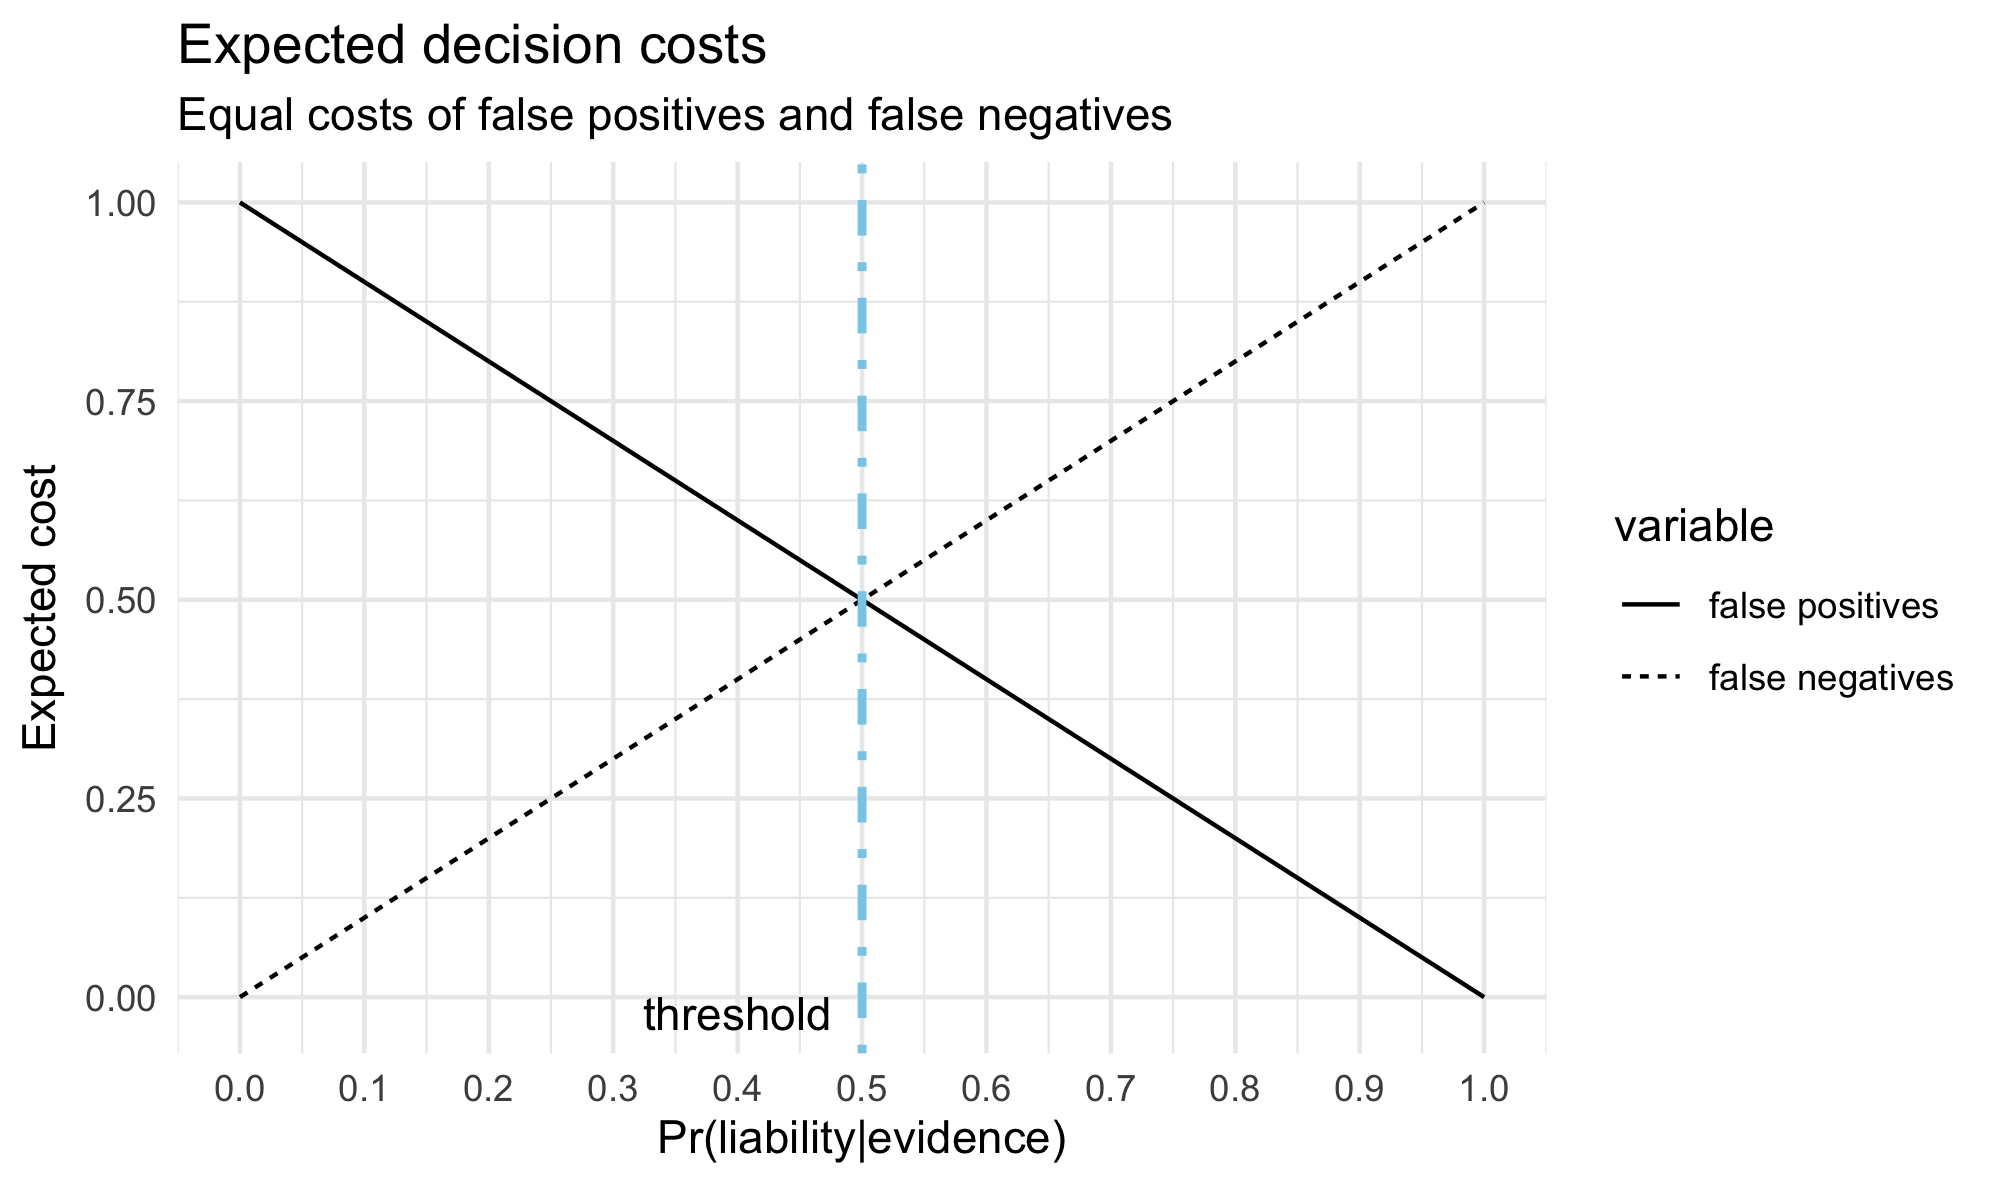
\includegraphics[width=10cm]{civil2.png}
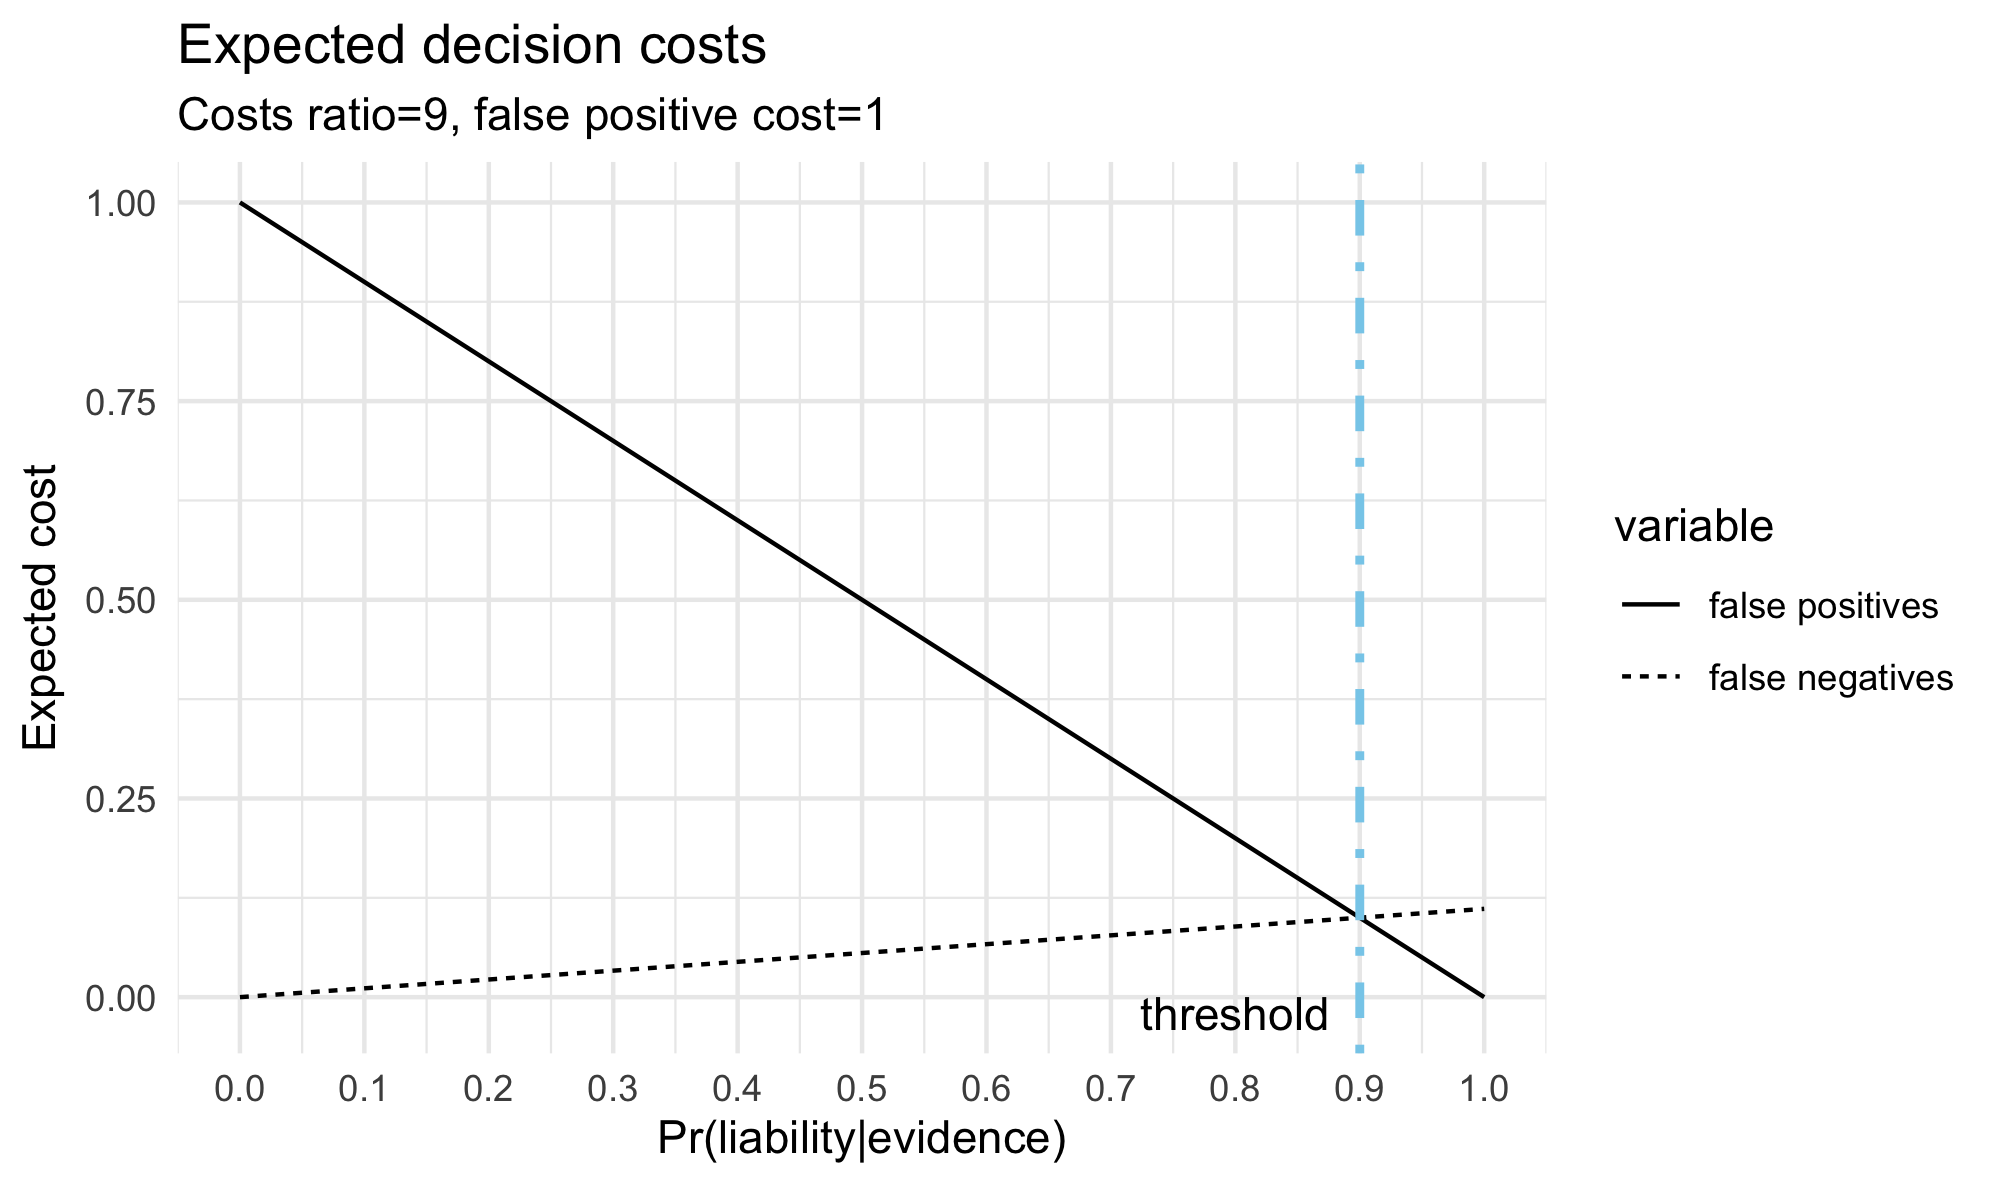
\includegraphics[width=10cm]{criminal4.png}   
\end{center}

This analysis only considers the costs of mistaken decisions, but leaves
out the benefits associated with correct decisions. More comprehensive
analyses would consider both. The basic insight remains the same,
however. The probability required for a conviction or a finding of civil
liability against the defendant is a function of weighing the costs and
benefits that would result from true and false positive as well as true
and false negative decisions. On this account of proof standards, the
stringency of the threshold depends on costs and benefits, and thus
different cases may require different thresholds. Cases in which the
charge is more serious than others---say, murder compared to petty
theft---may require higher thresholds so long as the cost of a mistaken
decision against the defendant is more significant. Standards of proof
would vary depending on the costs at stake in different cases. Whether
or not standards of proof should vary in this way is a matter of debate
{[}Kaplow (2012), Picinali (2013)\}. The same standard of proof is
typically applied for murder and petty theft. The law typically makes
coarse distinctions between standards of proof, such as `proof beyond a
reasonable doubt' for criminal cases, `preponderance of the evidence'
for civil cases and `clear and convincing evidence' for a narrow subset
of civil cases in which the accusation against the defendant is
particularly serious. Another complication is that eliciting costs and
benefits that result from trial decisions is not easy. Should they be
elicited through a democratic process or should different jurors or
judges apply their own in a subjective fashion? (CITE WHAT?) No matter
the answer to these questions, when probabilistic standards of proof are
paired with expected utility theory, they become part of the calculus of
utilities. In line with the law and economics movement, trial
decision-making is viewed as one instrument among others for maximizing
overall social welfare (Posner, 1973).

\hypertarget{minimizing-overall-expected-errors}{%
\subsection{Minimizing overall expected
errors}\label{minimizing-overall-expected-errors}}

Instead of thinking in terms of maximizing expected utility (or
minimizing expected costs), probabiListic standardS of proof can be also
be viewd more directly as regulating the rate of erroneous trial
decisions. We will see, however, that the error-centered approch agrees
to a large extent with the approach based on maximizing expected
utility.

Consider an idealized model of a criminal trial system.\\
Each defendant is assigned a probability \(x\) of criminal liability (or
guilt) based on the evidence presented at trial. Since over a period of
time many defendants face charges, the guilt probability will have its
own distribution. Extreme guilt probabilities set at 0\% or 100\%,
presumably, are assigned rarely in trials if ever, while values between
40\% and 80\% are more common.\\
A rigorous way to express this distribution is by means of a probability
density function, call it \(f(x)\).\\
The figure below uses a right skewed distribution
\(\textsf{beta(18,3)}\).

\begin{center}
    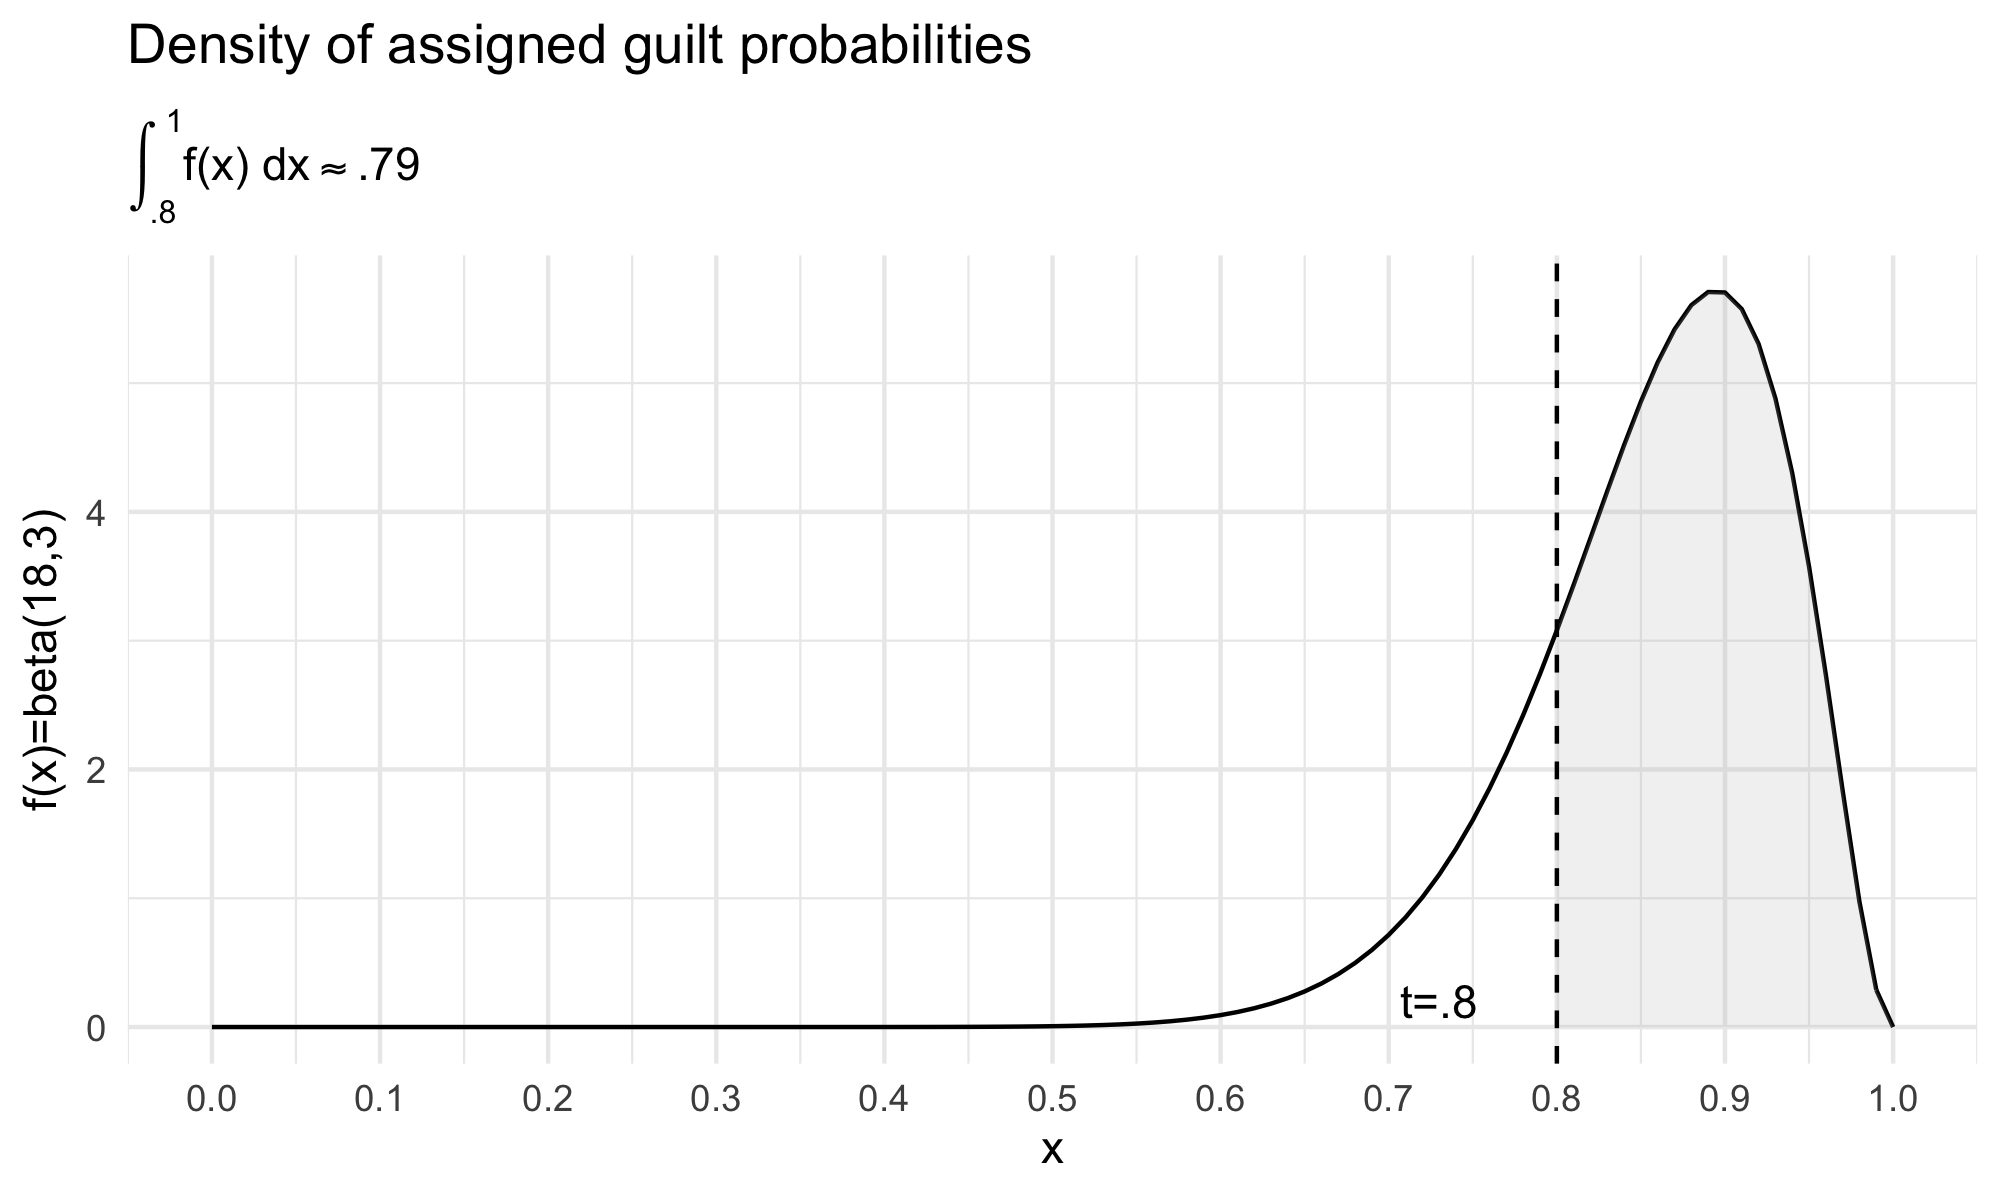
\includegraphics[width=10cm]{beta(18,3)2.png}
\end{center}

\noindent The right skew reflects the assumption that defendants in
criminal cases are sent to trial only if the incriminating evidence
against them is strong. It should be no surprise that most defendants
are assigned a high probability of guilt. The distribution of the
probability of liability in civil cases over a period of time might look
quite different, probably centered around 50\% or 60\%.

In the figure above, the threshold for conviction is set at \(>80\%\),
and the area under the curve to the right of the threshold is about
\(.79\). In other words, according to this model, 79\% of defendants on
trial are convicted and 21\% acquitted. These figures are close to the
rates of conviction and acquittal in many countries. Since \(f(x)\) is a
probability density, the total area under the curve adds up to 100\%,
encompassing all defendants, both convicted and acquitted defendants.

If the threshold becomes more stringent---for example, it moves up to
85\%---the rate of conviction would decrease provided the underlying
distribution does not change. But if the distribution becomes more
skewed toward the right---say \textsf{beta(25,3)}---the rate of
conviction could still be about 79\% even with a more stringent
threshold of 85\%.

\begin{center}
    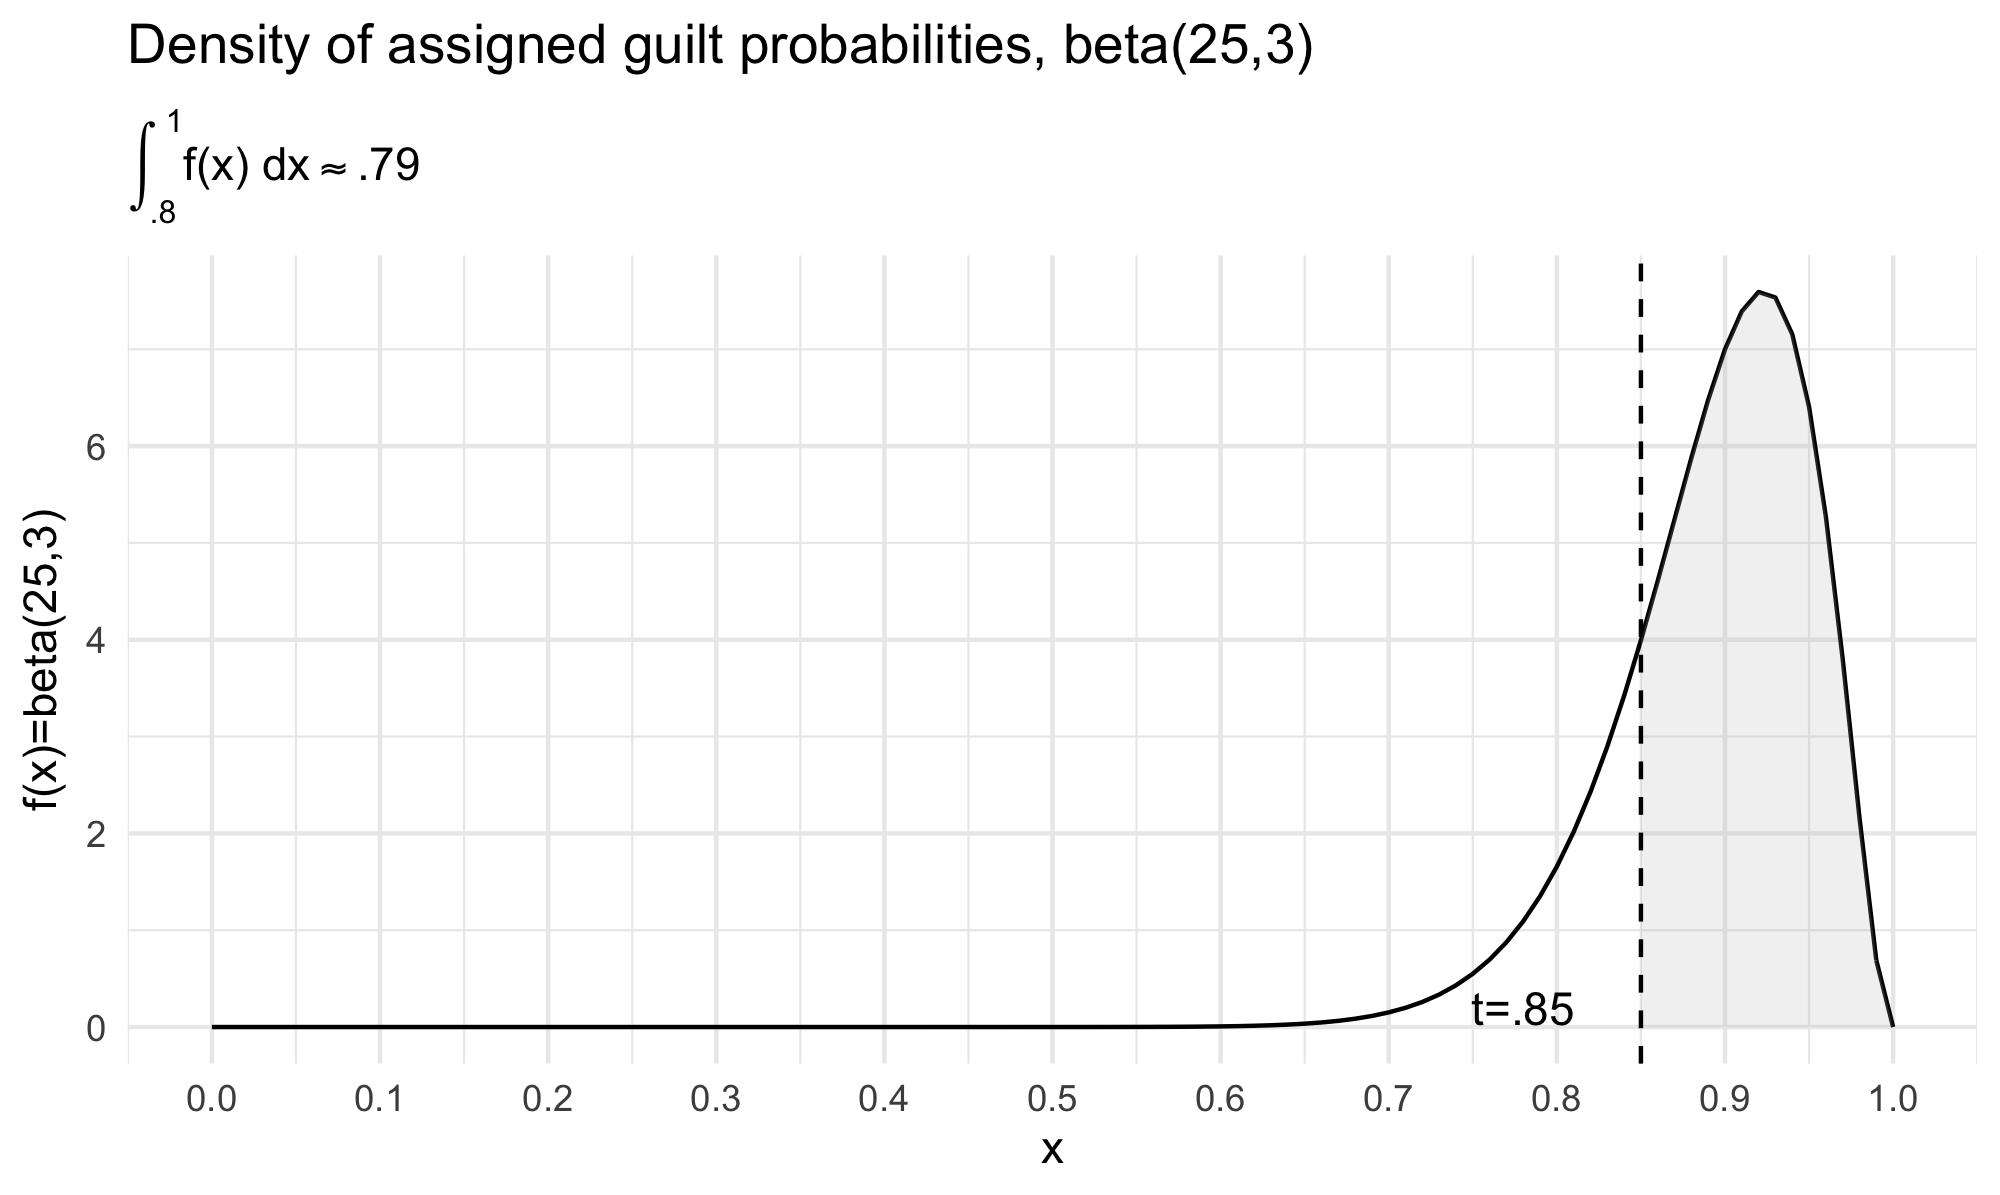
\includegraphics[width=10cm]{dbeta(25,3)2.png}
\end{center}

So far the model only describes the rate at which defendants are
convicted depending on the strigency of the threshold. But it is also
possible to represent in the model the rate at which innocent and guilty
defedants are convicted.

Presumably, among the defendants facing trail, some are factually
innocent and the rest are factually guilty. What is the proportion of
innocent and guilty defendants among all defendants? The expected
proportion of guilty and innocent defendants on trial, out of all
defendants, can be inferred from the density distribution \(f(x)\) under
certain assumptions. Suppose each defendant is assigned a guilt
probability based on the best and most complete evidence. From the
perspective of judges and jurors (or anyone who has access to the
evidence and evaluates it the same way), \(x\%\) of defendants who are
assigned \(x\%\) guilt probability are expected to be guilty and
\((1-x)\%\) innocent. For example, 85\% of defendants who are assigned a
85\% guilt probability are expected to be guilty and 15\% innocent; 90\%
of defendants who are assigned a 90\% guilt probability are expected to
be guilty and 10\% innocent; and so on.

Consequently, the function \(xf(x)\) describes the (expected) assignment
of guilt probabilities for guilty defendants, and similarly,
\((1-x)f(x)\) the (expected) assignment of guilt probabilities for
innocent defendants. Neither of these functions is a probability
density, since \(\int_0^1 \! xf(x) \, \mathrm{d}x=0.86\) and
\(\int_0^1 \! (1-x)f(x) \, \mathrm{d}x=0.14\). That is, the total areas
under the curve are, respectively, \(.86\) and \(.14\) (see graphs
below). These numbers express the (expected) proportion of guilty and
innocent defendants out of all defendants on trial, respectively 86\%
and 14\%.

The rates of incorrect decisions---false convictions and false
acquittals or more generally false positives and false negatives---can
be inferred from this model as a function of the threshold \(t\) (Hamer,
2004, @hamer2014). The integral \(\int_0^t \! xf(x) \, \mathrm{d}x\)
equals the expected rate of false acquittals, or in other words, the
expected proportion of guilty defendants who fall below threshold \(t\)
(out of all defendants), and the integral
\(\int_t^1 \! (1-x)f(x) \, \mathrm{d}x\) equals the expected rate of
false convictions, or in other words, the expected proportion of
innocent defendants who fall above threshold \(t\) (out of all
defendants). The rates of correct decisions---true convictions and true
acquittals or more generally true positives and true negatives---can be
inferred in a similar manner. The integral
\(\int_t^1 \! xf(x) \, \mathrm{d}x\) equals the expected rate of true
convictions and \(\int_0^t \! (1-x)f(x) \, \mathrm{d}x\) the expected
rate of true acquittals. In the figure below, the regions shaded in gray
correspond to false negatives (false acquittals) and false positives
(false convictions). The remaining white regions within the solid black
curve correspond to true positives (true convictions) and true negatives
(true acquittals). Note that the dotted blue curve is the original
overall distribution for all defendants.

\begin{center}
    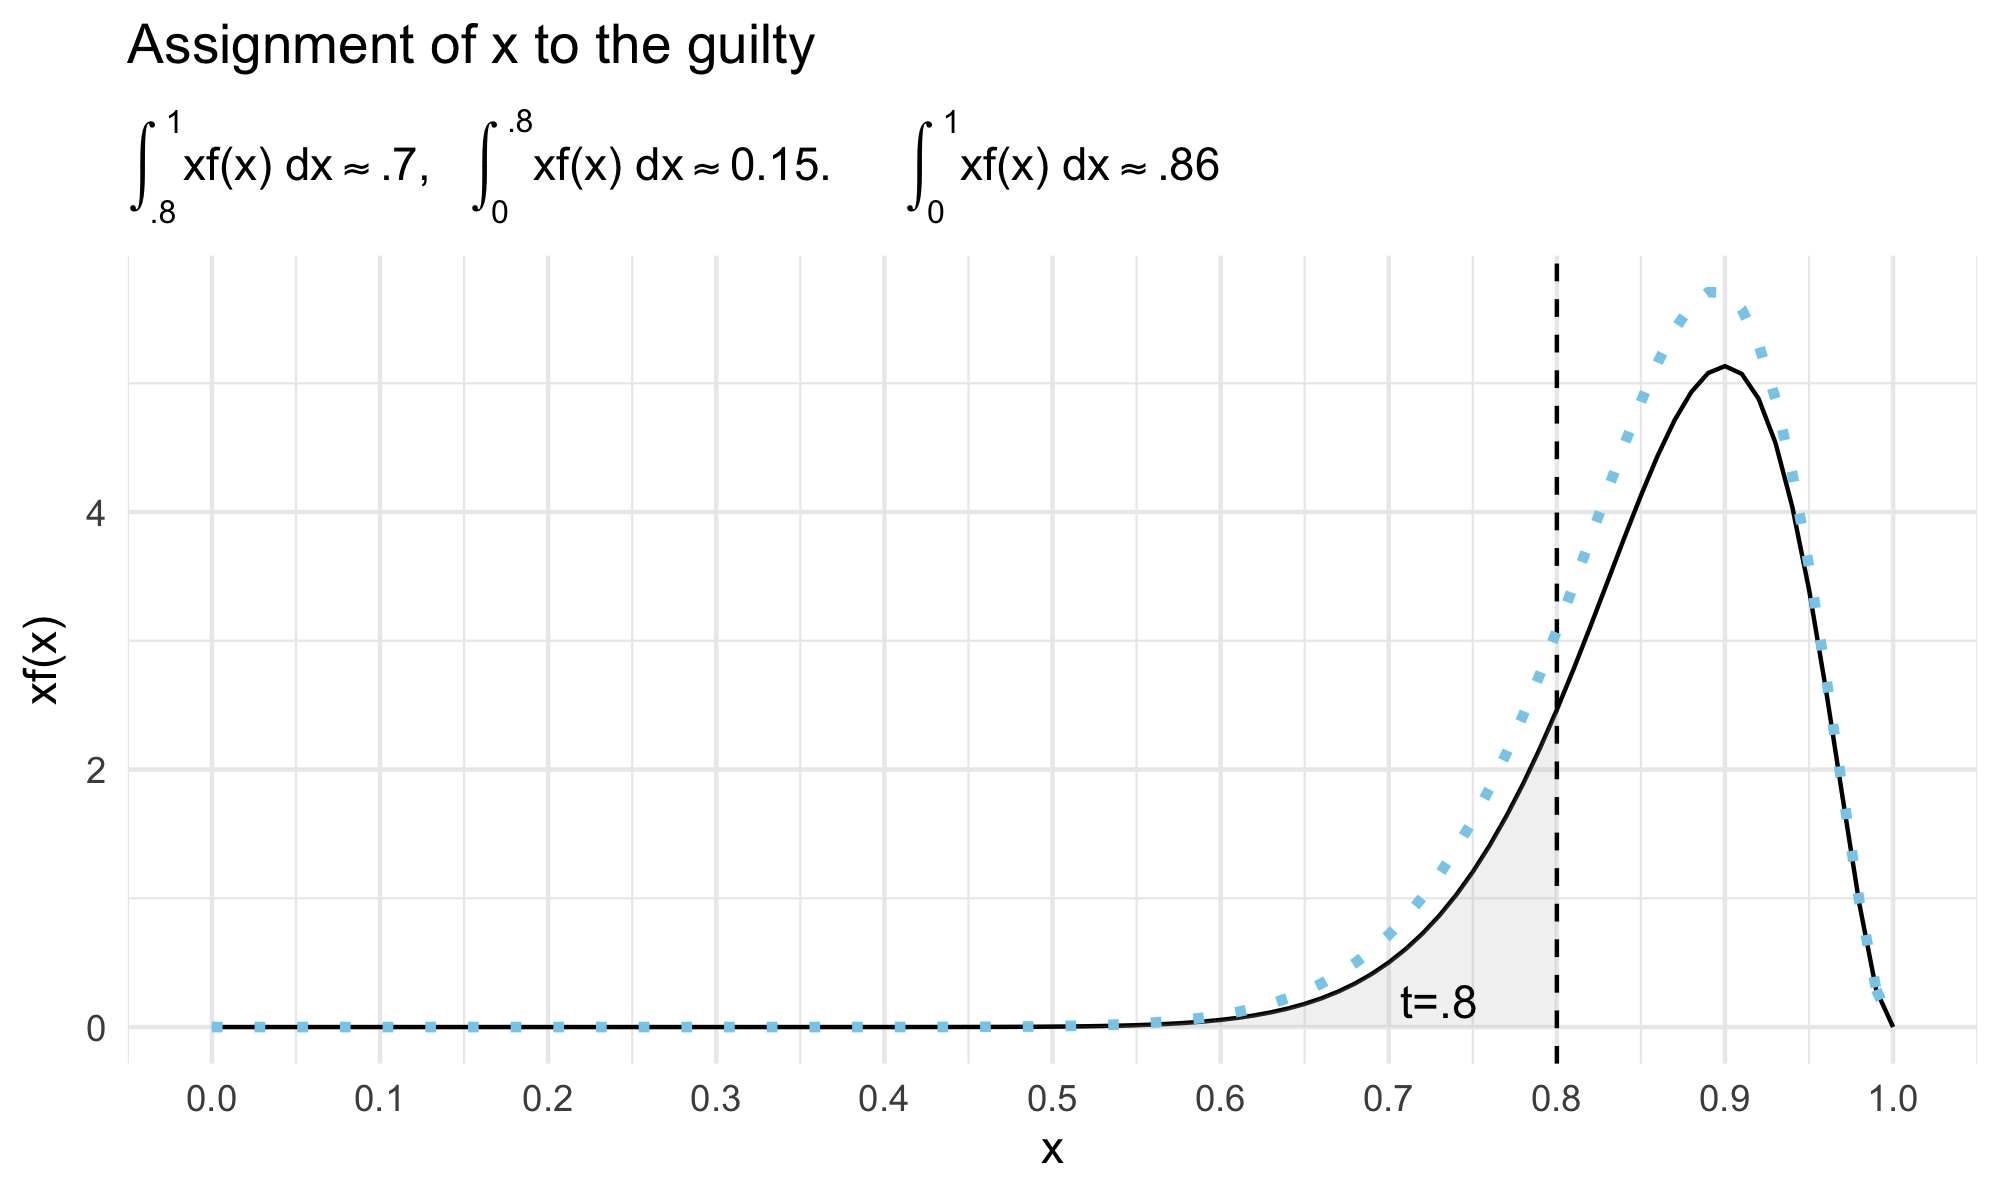
\includegraphics[width=10cm]{xfx3.png}
\end{center}

\begin{center}
    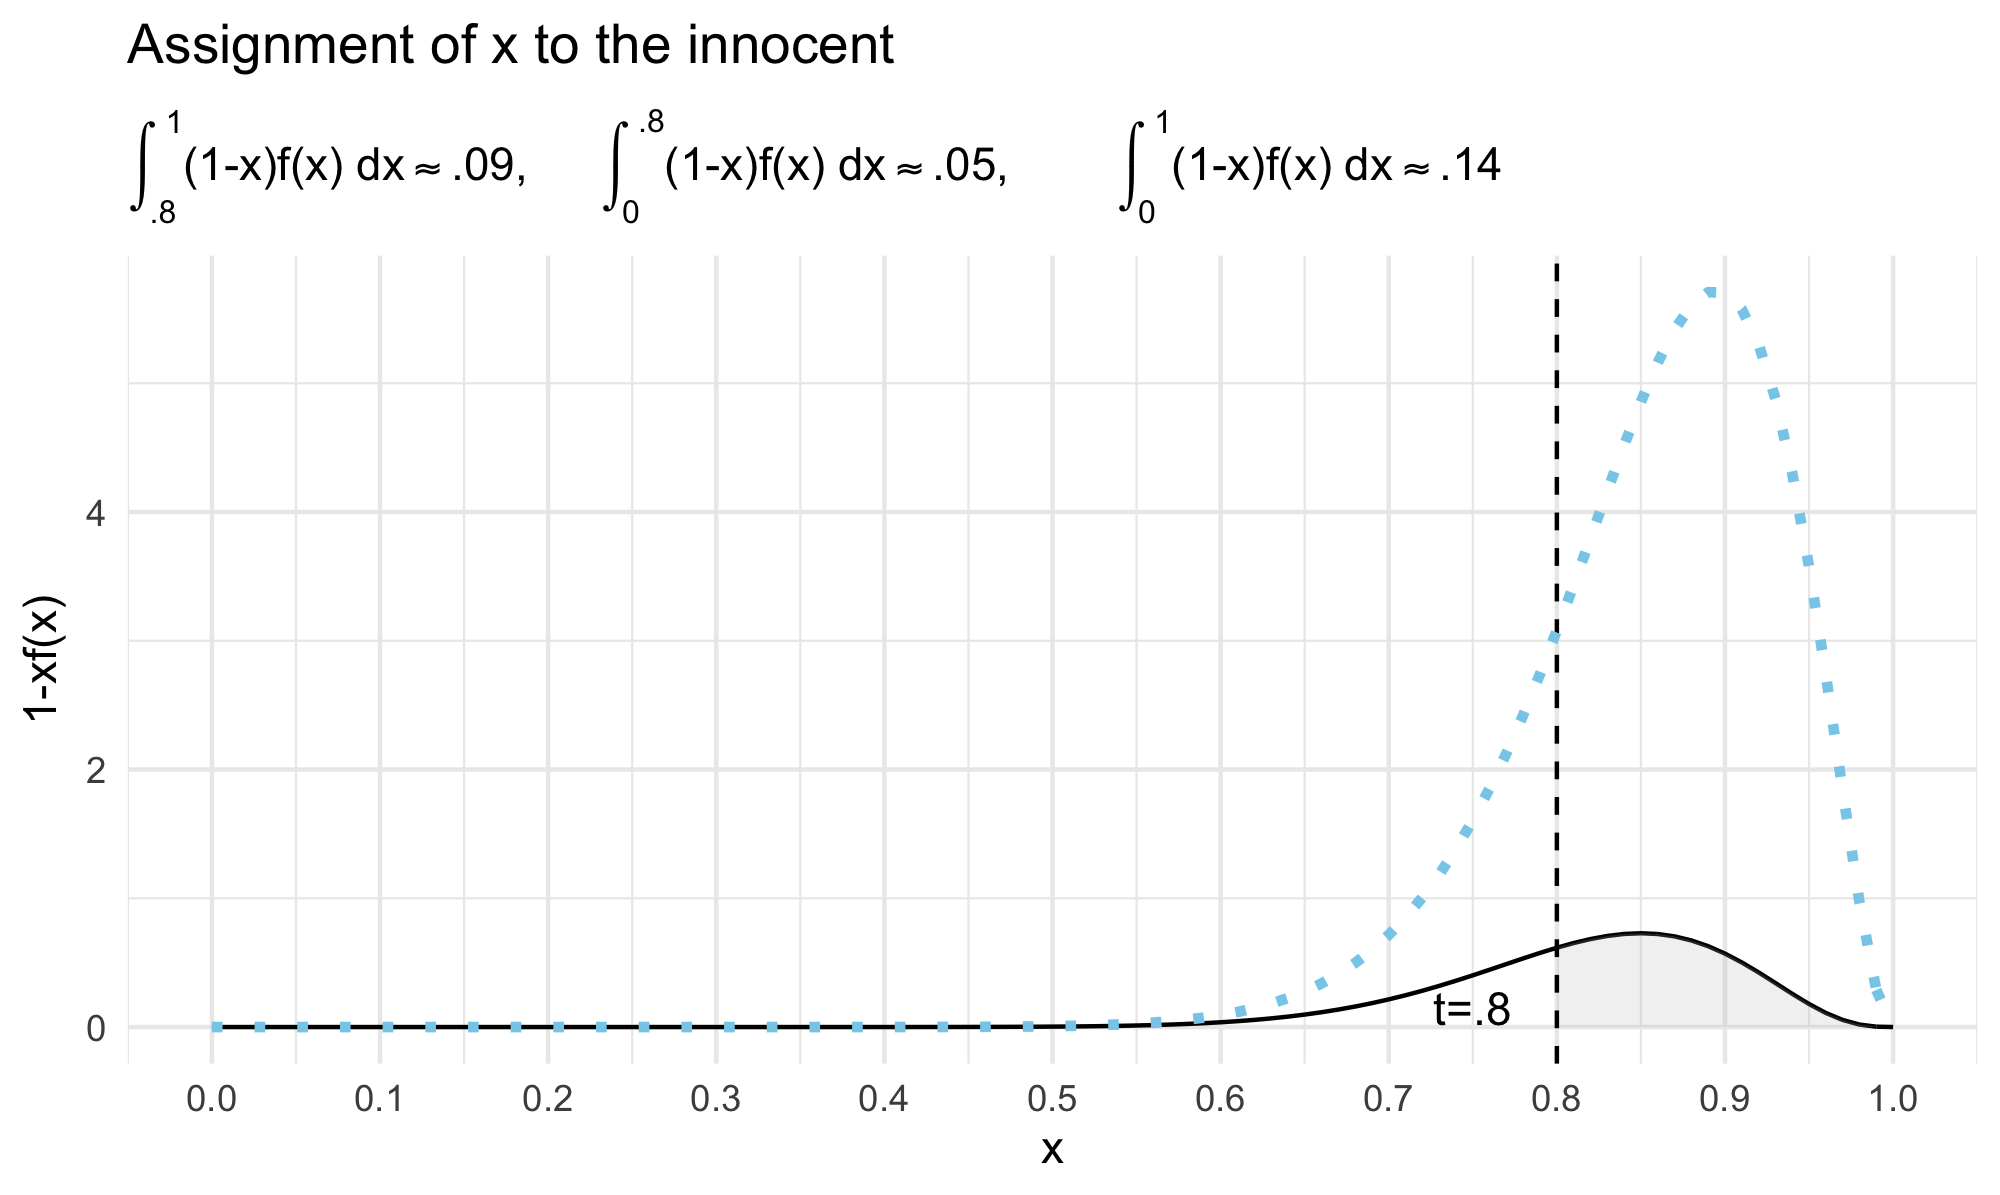
\includegraphics[width=10cm]{nxfx3.png}
\end{center}

The size of the grey regions in the figures above---which correspond to
false positives and false negatives---is affected by the location of
threshold \(t\). As \(t\) moves upwards, the rate of false positives
decreases but the rate of false negatives increases. Conversely, as
\(t\) moves downwards, the rate of false positives increases but the
rate of false negatives decreases. This trade-off is inescapable so long
as the underlying distribution is fixed. Below are both error
rates---false positives and false negatives---and their sum plotted
against a choice of \(t\), while holding fixed the ensity function
\(\textsf{binom(18,3)}\). The graph shows that any threshold that is no
greater than 50\% would minimize the total error rate (comprising false
positives and false negatives). A more stringent threshold, say
\(>90\%\), would instead significantly reduce the rate of false
positives but also significantly increase the rate of false negatives,
es expected.

\begin{center}
    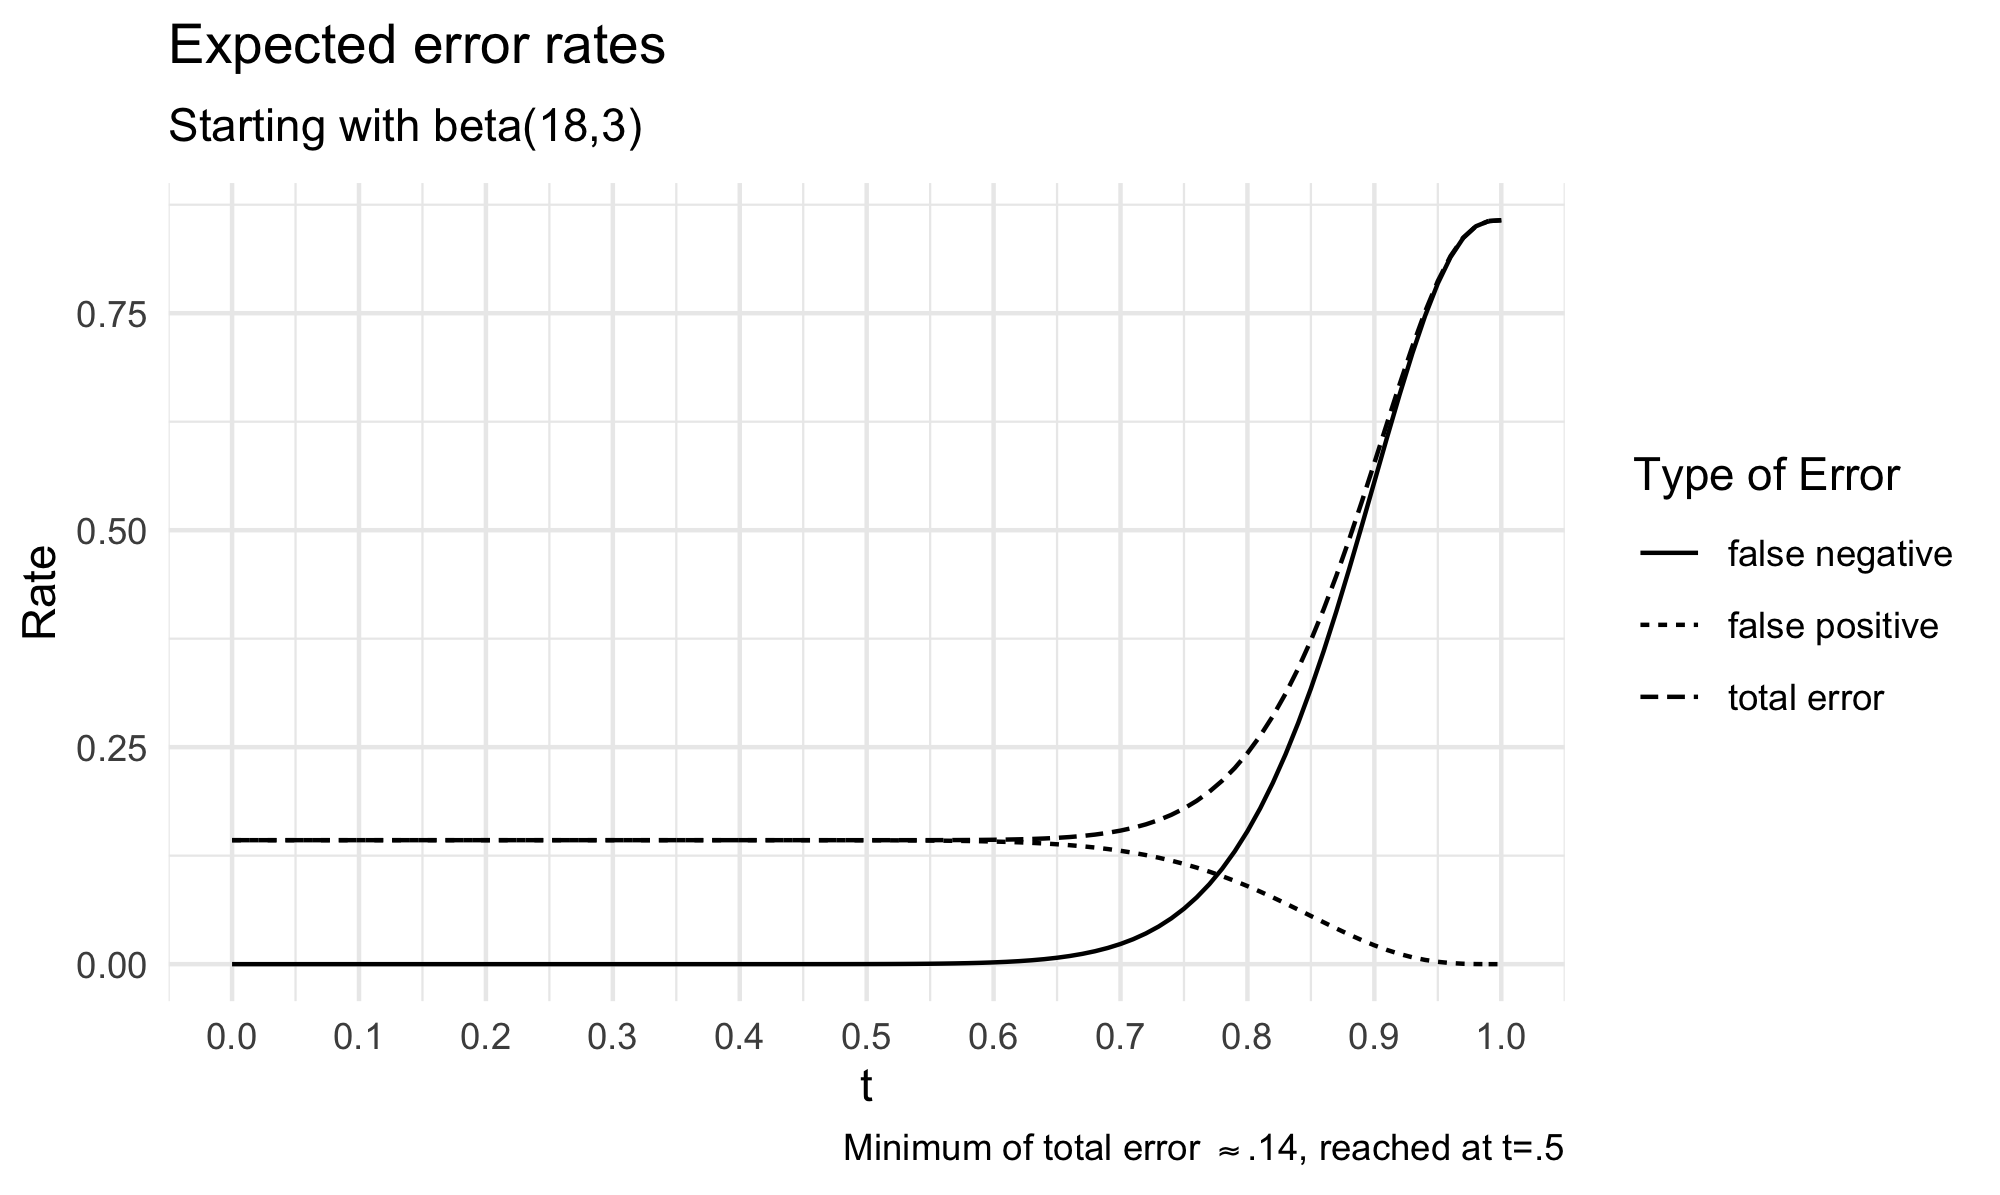
\includegraphics[width=12cm]{errors.png}
\end{center}

In general, the threshold that minimizes the expected rate of incorrect
decisions overall, no matter the underlying distribution, lies at
\(50\%\). The claim that setting threshold at \(t=.5\) minimizes the
expected error rate for any underlying distribution of \(x\) is general
and holds for \(t=.5\) only. It holds given the distribution
\(f(x)=\)beta(18,3) as well as any other distribution (Kaye, 1982,
@Kaye1999clarifying, @cheng2015). To show this, let \(E(t)\) as a
function of threshold \(t\) be the sum of rates of false positive and
false negative decisions:

\[E(t) = \int_0^t \! x f(x) \, \mathrm{d}x + \int_t^1 \! (1-x) f(x) \, \mathrm{d}x.
\]

The overall rate of error is minimized when \(E(t)\) is the lowest. To
determine the value of \(t\) for which \(E(t)\) is the lowest, set the
derivative of \(E(t)\) \%and \(R(t)\) to zero, that is,
\(\frac{d}{dt} E(t)= 0\). By calculus,
\(t=1/2\).\footnote{Note that $\frac{d}{dt}  E(t)$ is the the sum of the derivatives of $\int_0^t \! x f(x) \, \mathrm{d}x$ 
and 
%$\int_t^1 \! x f(x) \, \mathrm{d}x$
$\int_t^1 \!(1-x) f(x) \, \mathrm{d}x$, that is,

\[\frac{d}{dt} E(t) = \frac{d}{dt}  \int_0^t \! x f(x) \, \mathrm{d}x + \frac{d}{dt}  \int_t^1 \! (1-x) f(x) \, \mathrm{d}x.\]

By the fundamental theorem of calculus, 

\[\frac{d}{dt}   \int_0^t \! x f(x) \, \mathrm{d}x = tf(t) \text{ and }
\frac{d}{dt}   \int_t^1 \! (1-x) f(x) \, \mathrm{d}x = -(1-t)f(t). \]

By plugging in the values, 

\[\frac{d}{dt}  E(t) = tf(t)  -(1-t)f(t). \]

Since $\frac{d}{dt}  E(t)= 0$, then $tf(t)  = (1-t)f(t)$
and thus
$t  = 1-t$, so 
$t  = 1/2$ or a $>50\%$ threshold.
}

So a threshold of 50\% is the one that minimizes the aggregate rate of
erroneous decisions.

This claims holds when the two decisional errors are assigned the same
weight, or in other words, the costs of false positives and false
negatives are symmetric. The \(>50\%\) threshold therefore should be
most suitable for civil trials. In criminal trials, however, false
convictions are typically considered significantly more costly than
false acquittals, say a cost ratio of 9:1 (but see Epps, 2015). The sum
of the two error rates can be weighted by their respective costs:

\[E(t) = \int_0^t \! x f(x) \, \mathrm{d}x + 9\int_t^1 \! (1-x) f(x) \, \mathrm{d}x.\]

Given a cost ratio of 9:1, the optimal threshold that minimizes the
(weighted) overall rate of error is no longer \(1/2\), but rather,
\(t=9/10=90\%\).\footnote{The proof is the same as before. Since $tf(t)  = 9(1-t)f(t)$, it follows that $t  = 9/10$.}
Whenever the decision threshold is more stringent than \(>50\%\), the
overall (unweighted) error minimization may be sacrificed to pursue
other goals, for example, protecting more innocents against mistaken
convictions, even at the cost of making a larger number of mistaken
trial decisions overall.

\hypertarget{expected-errors-and-actual-errors}{%
\subsection{Expected errors and actual
errors}\label{expected-errors-and-actual-errors}}

The standard `proof beyond a reasonable doubt' is often paired with the
Blackstone ratio, the principle that it is better that ten guilty
defendants go free rather than even just one innocent be convicted. The
exact ratio is a matter of controversy (Volokh, 1997). It is tempting to
think that, say, a 99\% threshold guarantees a 1:99 ratio between false
convictions and false acquittals. But this would be hasty for at least
two reasons. First, probabilistic thresholds affect the expected rate of
mistaken decisions. The actual rate may deviate from its expected value
(Kaye, 1999). Second, if the threshold is \(99\%\), \textit{at most} 1\%
of decision against defendants are expected to be mistaken (false
convictions) and \textit{at most} 99\% of the decisions in favor of the
defendant are expected to be mistaken (false acquittals). The exact
ratio will depend on the probabilities assigned to defendants and how
they are distributed (Allen, 2014). The (expected) rate of false
positives and false negatives---and thus their ratio---depend on where
the threshold is located but also on the distribution of the liability
probability as given by the density function \(f(x)\).

\hypertarget{minimizing-mistaken-decisions}{%
\subsection{Minimizing mistaken
decisions}\label{minimizing-mistaken-decisions}}

\hypertarget{conclusion-1}{%
\section{Conclusion}\label{conclusion-1}}

\hypertarget{references}{%
\section*{References}\label{references}}
\addcontentsline{toc}{section}{References}

\hypertarget{refs}{}
\leavevmode\hypertarget{ref-allen2014}{}%
Allen, R. J. (2014). Burdens of proof. \emph{Law, Probability and Risk},
\emph{13}, 195--219.

\leavevmode\hypertarget{ref-Bernoulli1713Ars-conjectandi}{}%
Bernoulli, J. (1713). \emph{Ars conjectandi}.

\leavevmode\hypertarget{ref-buchak2014belief}{}%
Buchak, L. (2014). Belief, credence, and norms. \emph{Philosophical
Studies}, \emph{169}(2), 285--311.

\leavevmode\hypertarget{ref-cheng2015}{}%
Cheng, E., \& Pardo, M. S. (2015). Accuracy, optimality and the
preponderance standard. \emph{Law, Probability and Risk}, \emph{14}(3),
193--212.

\leavevmode\hypertarget{ref-davidsonpargetter1987}{}%
Davidson, B., \& Pargetter, R. (1987). Guilt beyond reasonable doubt.
\emph{Australasian Journal of Philosophy}, \emph{65}(2), 182--187.

\leavevmode\hypertarget{ref-Dekay1996}{}%
Dekay, M. L. (1996). The difference between Blackstone-like error ratios
and probabilistic standards of proof. \emph{Law and Social Inquiry},
\emph{21}, 95--132.

\leavevmode\hypertarget{ref-dhamiEtAl2015}{}%
Dhami, M. K., Lundrigan, S., \& Mueller-Johnson, K. (2015). Instructions
on reasonable doubt: Defining the standard of proof and the jurors task.
\emph{Psychology, Public Policy, and Law, 21(2), 169178}, \emph{21}(2),
169--178.

\leavevmode\hypertarget{ref-diamond90}{}%
Diamond, H. A. (1990). Reasonable doubt: To define, or not to define.
\emph{Columbia Law Review}, \emph{90}(6), 1716--1736.

\leavevmode\hypertarget{ref-epps2015}{}%
Epps, D. (2015). The consequences of error in criminal justice.
\emph{Harvard Law Review}, \emph{128}(4), 1065--1151.

\leavevmode\hypertarget{ref-finkelstein1970bayesian}{}%
Finkelstein, M. O., \& Fairley, W. B. (1970). A bayesian approach to
identification evidence. \emph{Harvard Law Review}, 489--517. JSTOR.

\leavevmode\hypertarget{ref-friedman1996}{}%
Friedman, R. D. (1996). Assessing evidence. \emph{Michigan Law Review},
\emph{94}, 1810--1838.

\leavevmode\hypertarget{ref-Friedman2000presumption}{}%
Friedman, R. D. (2000). A presumption of innocence, not of even odds.
\emph{Stanford Law Review}, \emph{52}(4), 873--887.

\leavevmode\hypertarget{ref-gardiner2019ppa}{}%
Gardiner, G. (2019). The reasonable and the relevant: Legal standards of
proof. \emph{Philosophy and Public Affairs}, \emph{47}(3), 288--318.

\leavevmode\hypertarget{ref-gordon2007}{}%
Gordon, T. F., Prakken, H., \& Walton, D. (2007). The Carneades model of
argument and burden of proof. \emph{Artificial Intelligence},
\emph{171}(10-15), 875--896.

\leavevmode\hypertarget{ref-Haack2014-HAAEMS}{}%
Haack, S. (2014). \emph{Evidence matters: Science, proof, and truth in
the law}. Cambridge University Press.

\leavevmode\hypertarget{ref-hamer2004}{}%
Hamer, D. (2004). Probabilistic standards of proof, their complements
and the errors that are expected to flow from them. \emph{University of
New England Law Journal}, \emph{1}(1), 71--107.

\leavevmode\hypertarget{ref-hamer2014}{}%
Hamer, D. (2014). Presumptions, standards and burdens: Managing the cost
of error. \emph{Law, Probability and Risk}, \emph{13}, 221--242.

\leavevmode\hypertarget{ref-hastie2019CaseRelativePlausibilitya}{}%
Hastie, R. (2019). The case for relative plausibility theory: Promising,
but insufficient. \emph{The International Journal of Evidence \& Proof},
\emph{23}(1-2), 134--140.

\leavevmode\hypertarget{ref-ho2008philosophy}{}%
Ho, H. L. (2008). \emph{A philosophy of evidence law: Justice in the
search for truth}. Oxford University Press.

\leavevmode\hypertarget{ref-lai2019HowPlausibleRelative}{}%
Ho, H. L. (2019). How plausible is the relative plausibility theory of
proof? \emph{The International Journal of Evidence \& Proof},
\emph{23}(1-2), 191--197.

\leavevmode\hypertarget{ref-Horowitz1996}{}%
Horowitz, I. A., \& Kirkpatrick, L. C. (1996). A concept in search of a
definition: The effect of reasonable doubt instrcutions on certainty of
guilt standards and jury verdicts. \emph{Law and Human Behaviour},
\emph{20}(6), 655--670.

\leavevmode\hypertarget{ref-Kaplan1968decision}{}%
Kaplan, J. (1968). Decision theory and the fact-finding process.
\emph{Stanford Law Review}, \emph{20}(6), 1065--1092.

\leavevmode\hypertarget{ref-kaplow2012}{}%
Kaplow, L. (2012). Burden of proof. \emph{Yale Law Journal},
\emph{121}(4), 738--1013.

\leavevmode\hypertarget{ref-kaye79}{}%
Kaye, D. H. (1979a). The laws of probability and the law of the land.
\emph{The University of Chicago Law Review}, \emph{47}(1), 34--56.

\leavevmode\hypertarget{ref-Kaye79gate}{}%
Kaye, D. H. (1979b). The paradox of the Gatecrasher and other stories.
\emph{The Arizona State Law Journal}, 101--110.

\leavevmode\hypertarget{ref-kaye1982limits}{}%
Kaye, D. H. (1982). The limits of the preponderance of the evidence
standard: Justifiably naked statistical evidence and multiple causation.
\emph{Law \& Social Inquiry}, \emph{7}(2), 487--516. Wiley Online
Library.

\leavevmode\hypertarget{ref-Kaye1986Do}{}%
Kaye, D. H. (1986). Do we need a calculus of weight to understand proof
beyond a reasonable doubt? \emph{Boston University Law Review},
\emph{66}, 657--672.

\leavevmode\hypertarget{ref-Kaye1999clarifying}{}%
Kaye, D. H. (1999). Clarifying the burden of persuasion: What Bayesian
rules do and not do. \emph{International Commentary on Evidence},
\emph{3}, 1--28.

\leavevmode\hypertarget{ref-Laplace1814}{}%
Laplace, P. (1814). \emph{Essai philosophique sur les probabilités}.

\leavevmode\hypertarget{ref-laudan2006truth}{}%
Laudan, L. (2006). \emph{Truth, error, and criminal law: An essay in
legal epistemology}. Cambridge University Press.

\leavevmode\hypertarget{ref-nance2016}{}%
Nance, D. A. (2016). \emph{The burdens of proof: Discriminatory power,
weight of evidence, and tenacity of belief}. Cambridge University Press.

\leavevmode\hypertarget{ref-nance2019LimitationsRelativePlausibility}{}%
Nance, D. A. (2019). The limitations of relative plausibility theory.
\emph{The International Journal of Evidence \& Proof}, \emph{23}(1-2),
154--160.

\leavevmode\hypertarget{ref-newman1993}{}%
Newman, J. O. (1993). Beyon ``reasonable doub''. \emph{New York
University Law Review}, \emph{68}(5), 979--1002.

\leavevmode\hypertarget{ref-Pardo2008judicial}{}%
Pardo, M. S., \& Allen, R. J. (2008). Judicial proof and the best
explanation. \emph{Law and Philosophy}, \emph{27}(3), 223--268.

\leavevmode\hypertarget{ref-Pennington1991}{}%
Pennington, N., \& Hastie, R. (1991). A cognitive theory of juror
decision making: The story model. \emph{Cardozo Law Review}, \emph{13},
519--557.

\leavevmode\hypertarget{ref-penn1993}{}%
Pennington, N., \& Hastie, R. (1993). Reasoning in explanation-based
decision making. \emph{Cognition}, \emph{49}, 123--163.

\leavevmode\hypertarget{ref-picinali2013}{}%
Picinali, F. (2013). Two meanings of ``reasonableness": Dispelling the
``floating" reasonable doubt. \emph{Modern Law Review}, \emph{76}(5),
845--875.

\leavevmode\hypertarget{ref-Posner1973}{}%
Posner, R. (1973). \emph{The economic analysis of law}. Brown \&
Company.

\leavevmode\hypertarget{ref-prakken2009}{}%
Prakken, H., \& Sartor, G. (2009). A logical analysis of burdens of
proof. In H. Kaptein, H. Prakken, \& B. Verheij (Eds.), \emph{Legal
evidence and proof: Statistics, stories, logic} (pp. 223--253). Ashgate.

\leavevmode\hypertarget{ref-schwartz2019WhatRelativePlausibility}{}%
Schwartz, D. S., \& Sober, E. (2019). What is relative plausibility?
\emph{The International Journal of Evidence \& Proof}, \emph{23}(1-2),
198--204.

\leavevmode\hypertarget{ref-stein2008}{}%
Stein, A. (2008). The right to silence helps the innocent: A reseponse
to critics. \emph{Cardozo Law Review}, \emph{30}(3), 1115--1140.

\leavevmode\hypertarget{ref-tribe71}{}%
Tribe, L. H. (1971). Trial by mathematics: Precision and ritual in the
legal process. \emph{Harvard Law Review}, \emph{84}(6), 1329--1393.

\leavevmode\hypertarget{ref-Urbaniak2017Narration-in-ju}{}%
Urbaniak, R. (2018). Narration in judiciary fact-finding: A
probabilistic explication. \emph{Artificial Intelligence and Law},
1--32.

\leavevmode\hypertarget{ref-voloch1997}{}%
Volokh, A. (1997). N guilty men. \emph{University of Pennsylvania Law
Review}, \emph{146}(2), 173--216.

\leavevmode\hypertarget{ref-walen2015}{}%
Walen, A. (2015). Proof beyond a reasonable doubt: A balanced
retributive account. \emph{Louisiana Law Review}, \emph{76}(2),
355--446.

\end{document}
